\documentclass[a4paper,12pt]{article}
\usepackage{graphicx} 
\usepackage{hyperref}
\usepackage{float}
\usepackage{booktabs}
\usepackage{longtable}
\usepackage{bookmark}
\usepackage{multirow}

% \begin{figure}[H]
%     \centering
%     \includegraphics[width=0.7\textwidth]{filename.png}
%     \caption{Your figure caption here.}
%     \label{fig:yourlabel}
% \end{figure}

\begin{document}

\title{Assignment 5 - Data Science\\
Insurance Policy Cost Prediction}
\author{Mohammad Hossein Basouli}
\date{\today}
\maketitle

\begin{center}
    \textit{\section*{Abstract}}
    \textit{In this analysis we try to study the factors that influence the policy cost determined by an insurance company. 
    Some key findings of this analysis are: \textit{Yearly Earnings}, \textit{Financial Rating}, \textit{Prior Claims}, 
    and \textit{Wellness Index} are the most influential factors in determination of \textit{Policy Cost}.}
\end{center}

% ---------------------------------------------------------------------------------------------------------------------------------------------------------------------------------------------------------------------- %

\section{Introduction}
\subsection{Background:} 
Correct determination of \textit{Policy Cost} is a crucial part of the work that insurance companies do everyday; And machine learning is a powerful tool that can be used in order to 
have an accurate prediction on this objective. In this analysis we work with a dataset gathered from an insurance company, which in turn, includes many valuable features about \textbf{Demographic}, 
\textbf{Health}, and \textbf{Finance} of the person whom is been giving service to, as well as, information about the \textbf{Property/Asset} itself. 

\subsection{Objectives:} 
Below provides the flow of our analysis in a nutshell:
\begin{enumerate}
    \item First we will try to gain a basic understanding about our data through \textbf{Exploratory Data Analysis} section.
    \item Then we will apply a preprocessing step, to ensure the quality of the data.
    \item Next, we shall apply different \textbf{Feature Engineering} techniques, in order to help our models, capture patterns from the data.
    \item After that, we are going to train our models and evaluate them and see which one performs the best.
    \item Then we shall extract the importances of the features, obtained by each of the models and try to provide useful insights for our business.
\end{enumerate}

\section{Data}
\subsection{An Overview:} 
The data has been gathered from a Kaggle competetion. The dataset includes 1.1 million and 21 columns in total. The features include both categorical (both nominal and ordinal) and continuous values. 

\subsection{Exploratory Data Analysis}
\subsubsection{Missing Values:}
The missing values for each of the columns are shown in the figure~\ref{fig:fig_1}.

\begin{figure}[H]
    \centering
    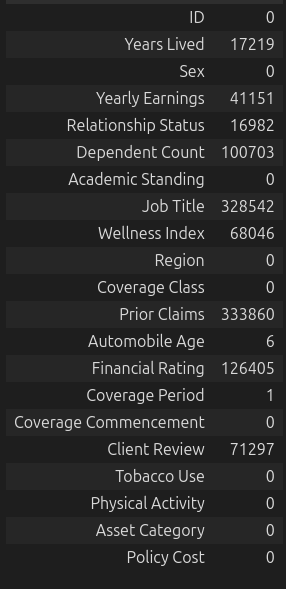
\includegraphics[scale=0.5]{./images/missing_values.png}
    \caption{Missing Values}
    \label{fig:fig_1}
\end{figure}

\subsubsection{Uni-Variate Analysis:}
We can see the distribution of all of the numerical features in the figure~\ref{fig:fig_2}; As you can see, the distribution of \textit{Yearly Earnings} is skewed to the right, 
but other features are distributed as normal or uniform.

\begin{figure}[H]
    \centering
    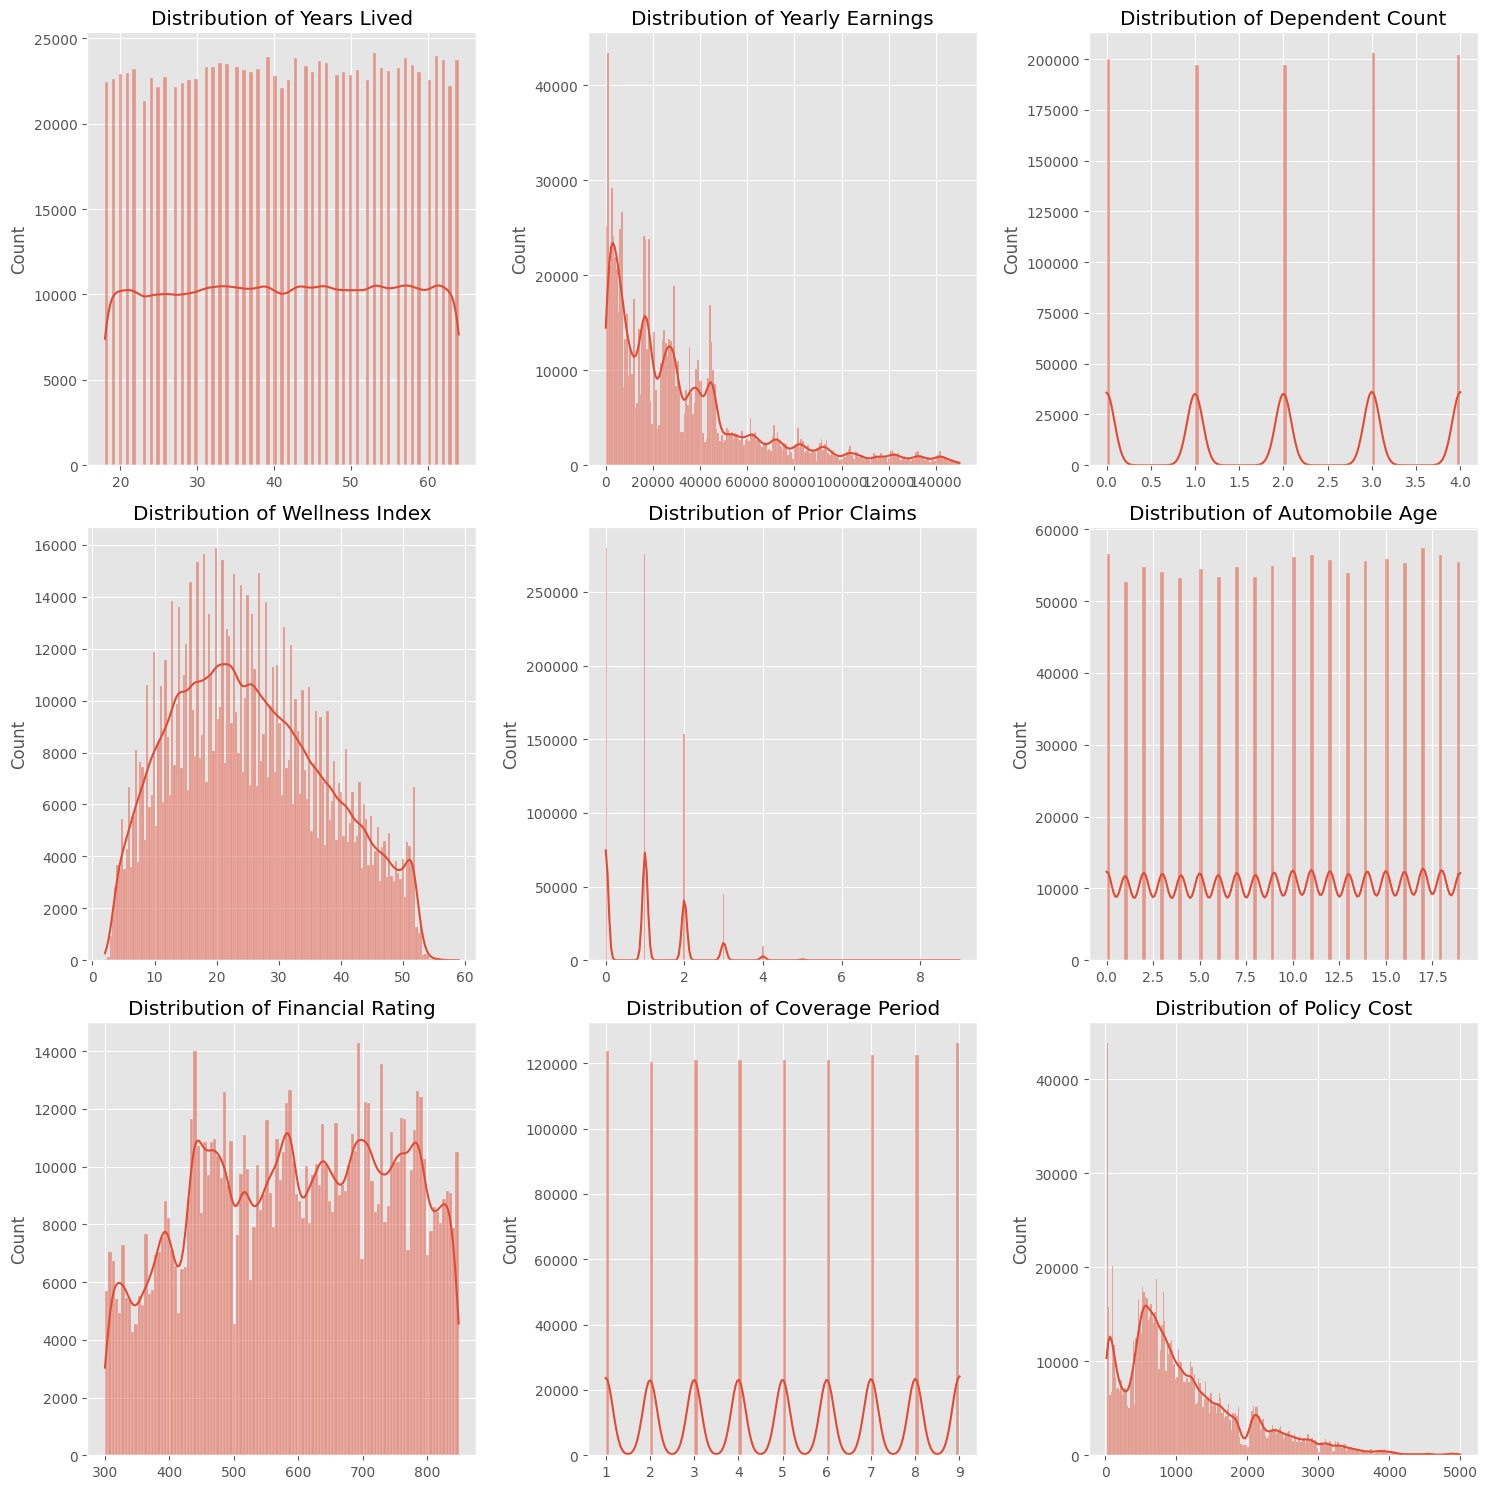
\includegraphics[width=\textwidth]{./images/univariate_anal.png}
    \caption{Distribution of Numerical Features}
    \label{fig:fig_2}
\end{figure}

\subsubsection{Bi-Variate Analysis:}
We can see the correlation matrix of all of the numerical features in the figure~\ref{fig:fig_3}; We observe that no pair of the features have a high correlation with each other. 

\begin{figure}[H]
    \centering
    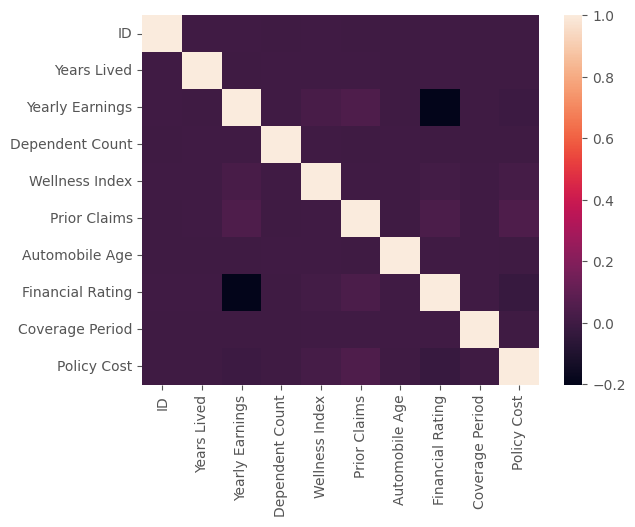
\includegraphics[width=\textwidth]{./images/bivariate_analysis.png}
    \caption{Heatmap of the Correlation Matrix}
    \label{fig:fig_3}
\end{figure}

\subsection{Data Preprocessing}
\subsubsection{Imputation of the Missing Values:}
We will impute the missing values by following the rule below:
\begin{itemize}
    \item \textbf{Datetime} \& \textbf{Categorical Features} $\rightarrow$ by Mode
    \item \textbf{Continuous Features} $\rightarrow$ by Median
\end{itemize}

\subsection{Feature Engineering}
\subsubsection{Feature Expansion:}
We will expand our features by extracting the following features from \textit{Coverage Commencement}:
\begin{itemize}
    \item \textit{CoverageCommencement\_Year}
    \item \textit{CoverageCommencement\_Month}
    \item \textit{CoverageCommencement\_DayOfWeek}
    \item \textit{CoverageCommencement\_DayOfYear}
    \item \textit{CoverageCommencement\_Season}
\end{itemize}

\subsubsection{Feature Transformation:}
We shall transform the feature, \textit{Yearly Earnings}, by \textbf{Square Root} function, in order to make it's distribution more normal.

\subsubsection{Feature Encodings:}
We will apply \textbf{Feature Encodings} as follows:
\begin{itemize}
    \item \textbf{Label Encodings:}
    \begin{itemize}
        \item \textit{Academic Standings}
        \item \textit{Coverage Class}
        \item \textit{Client Review}
        \item \textit{Physical Activity}
    \end{itemize}
    
    \item \textbf{Target Encodings (with cross validation):}
    \begin{itemize}
        \item \textit{Sex}
        \item \textit{Relationship Status}
        \item \textit{Job Title}
        \item \textit{Region}
        \item \textit{Tobacco Use}
        \item \textit{Asset Category}
        \item \textit{CoverageCommencement\_DayOfWeek}
        \item \textit{CoverageCommencement\_Season}
    \end{itemize}
\end{itemize}

\section{Models \& Evaluation}
\subsection{Splitting:}
We will use 80\% of the data as train, and 20\% as validation.

\subsection{Subsampling:}
We shall use 1\% of the data to decide on the best hyperparameters. Also we shall re-train and evaluate the models with the best hyperparameters with only a 5\% of the train and validation set.

\subsection{Evaluation Metric:}
We will use the metric \textbf{RMSLE} to evalate our models. The formula is given below:
\[
RMSLE = \sqrt{ \frac{1}{n} \sum_{i=1}^{n} \left( \log(1 + \hat{y}_i) - \log(1 + y_i) \right)^2 }
\]

\subsection{Models:}
The models that we will use in this analysis are as follows:
\begin{enumerate}
    \item \textbf{Random Forests}
    \item \textbf{AdaBoost}
    \item \textbf{XGBoost}
    \item \textbf{Light Boost}
    \item \textbf{Cat Boost}
    \item \textbf{Polynomial Regression with Ridge Regularization}
\end{enumerate}

\subsection{Hyperparameter Tuning:}
The results of \textbf{Hyperparameter Tuning} for each of the models is as follows:
\subsubsection{Random Forests}
\begin{figure}[H]
    \centering
    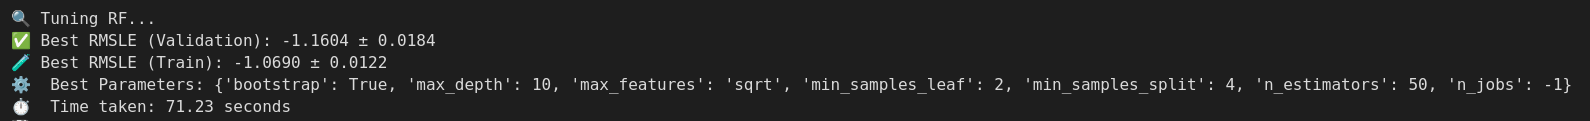
\includegraphics[width=\textwidth]{./images/rf_hyper.png}
    \caption{Hyperparameter Tuning Results for Random Forests}
    \label{fig:fig_4}
\end{figure}

\subsubsection{AdaBoost}
\begin{figure}[H]
    \centering
    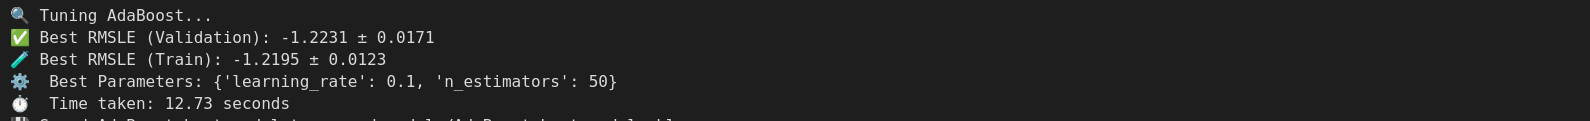
\includegraphics[width=\textwidth]{./images/ada_hyper.png}
    \caption{Hyperparameter Tuning Results for AdaBoost}
    \label{fig:fig_5}
\end{figure}

\subsubsection{XGBoost}
\begin{figure}[H]
    \centering
    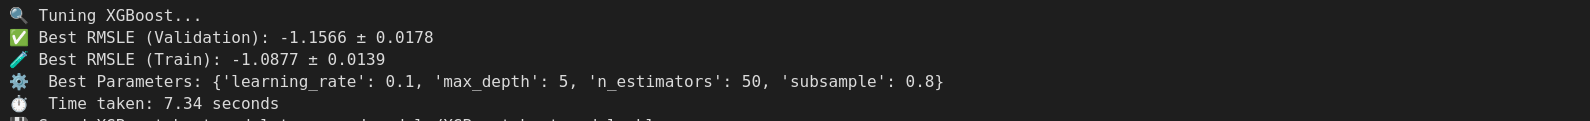
\includegraphics[width=\textwidth]{./images/xg_hyper.png}
    \caption{Hyperparameter Tuning Results for XGBoost}
    \label{fig:fig_6}
\end{figure}

\subsubsection{Light Gradient Boost}
\begin{figure}[H]
    \centering
    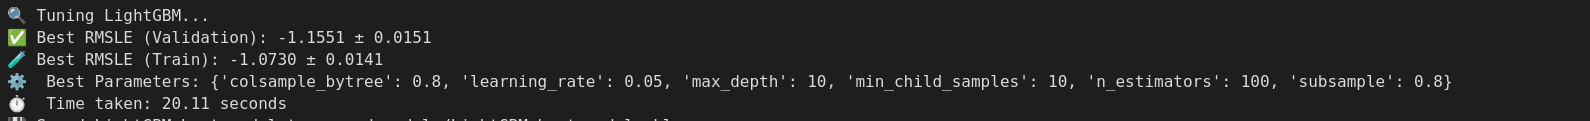
\includegraphics[width=\textwidth]{./images/light_hyper.png}
    \caption{Hyperparameter Tuning Results for Light Gradient Boost}
    \label{fig:fig_7}
\end{figure}

\subsubsection{Cat Boost}
\begin{figure}[H]
    \centering
    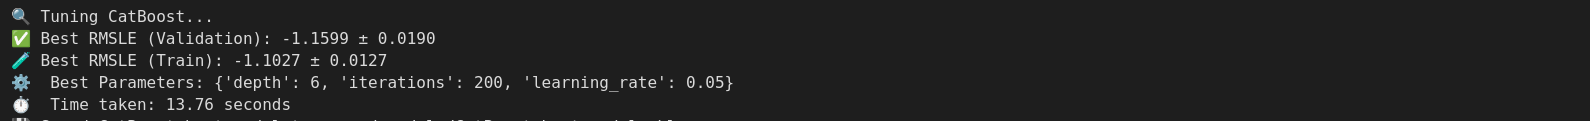
\includegraphics[width=\textwidth]{./images/cat_hyper.png}
    \caption{Hyperparameter Tuning Results for Cat Boost}
    \label{fig:fig_8}
\end{figure}

\subsubsection{Polynomial Regression with Ridge Regularization}
\begin{figure}[H]
    \centering
    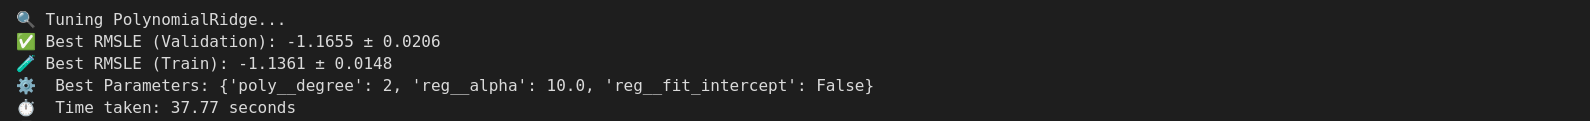
\includegraphics[width=\textwidth]{./images/polyridg_hyper.png}
    \caption{Hyperparameter Tuning Results for Polynomial Regression with Ridge Regularization}
    \label{fig:fig_9}
\end{figure}

\subsection{Re-Training \& Evaluation}
The results obtained after re-training and then evaluation can be seen in the table~\ref{tab:tab_1}.
\begin{table}[h!]
\centering
\begin{tabular}{|l|c|c|}
\hline
\textbf{Model} & \textbf{Train RMSLE} & \textbf{Validation RMSLE} \\
\hline
AdaBoost         & 1.2418 & 1.2315 \\
CatBoost         & 1.1518 & 1.1499 \\
LightGBM         & 1.1385 & 1.1416 \\
PolynomialRidge  & 1.1636 & 1.1561 \\
RF               & 1.1365 & 1.1543 \\
XGBoost          & 1.1459 & 1.1485 \\
\hline
\end{tabular}
\caption{RMSLE scores for each of the models on training and validation sets after re-training.}
\label{tab:tab_1}
\end{table}


\subsection{Feature Importances}
As we can see in the table~\ref{tab:tab_2}, \textit{Yearly Earnings}, \textit{Financial Rating}, \textit{Prior Claims}, \textit{CoverageCommencement\_DayOfYear} and 
\textit{Wellness Index} are among the most 10 influential features, across most of the models. We will provide insights about how these feature importances are going to help our business in the next section.
\begin{table}[H]
\centering
\caption{Top 10 Feature Importances per Model}
\label{tab:feature_importances}
\resizebox{\textwidth}{!}{%
\renewcommand{\arraystretch}{0.9}
\begin{tabular}{|l|l|c|}
\hline
\textbf{Model} & \textbf{Feature} & \textbf{Importance} \\
\hline
\multirow{10}{*}{CatBoost (Impurity)} 
  & Yearly Earnings & 23.3703 \\
  & Financial Rating & 13.9649 \\
  & Prior Claims & 12.2697 \\
  & Wellness Index & 7.4267 \\
  & CoverageCommencement\_Year & 7.3464 \\
  & Automobile Age & 3.1645 \\
  & CoverageCommencement\_DayOfWeek & 2.7919 \\
  & Years Lived & 2.6373 \\
  & Client Review & 2.5793 \\
  & Physical Activity & 2.2474 \\
\hline
\multirow{10}{*}{XGBoost (Impurity)} 
  & CoverageCommencement\_Year & 0.1165 \\
  & Prior Claims & 0.0833 \\
  & Yearly Earnings & 0.0640 \\
  & Financial Rating & 0.0623 \\
  & Wellness Index & 0.0484 \\
  & Physical Activity & 0.0450 \\
  & Client Review & 0.0435 \\
  & CoverageCommencement\_DayOfWeek & 0.0395 \\
  & Coverage Period & 0.0389 \\
  & CoverageCommencement\_DayOfYear & 0.0378 \\
\hline
\multirow{10}{*}{Polynomial Ridge (Permutation)} 
  & CoverageCommencement\_Month & 0.0998 \\
  & CoverageCommencement\_DayOfYear & 0.0877 \\
  & Yearly Earnings & 0.0103 \\
  & Financial Rating & 0.0085 \\
  & Prior Claims & 0.0081 \\
  & CoverageCommencement\_Year & 0.0055 \\
  & Dependent Count & 0.0019 \\
  & CoverageCommencement\_Season & 0.0018 \\
  & Sex & 0.0016 \\
  & Tobacco Use & 0.0016 \\
\hline
\multirow{10}{*}{Random Forest (Impurity)} 
  & Yearly Earnings & 0.1679 \\
  & Financial Rating & 0.1149 \\
  & Wellness Index & 0.0993 \\
  & CoverageCommencement\_DayOfYear & 0.0831 \\
  & Years Lived & 0.0657 \\
  & Automobile Age & 0.0553 \\
  & Prior Claims & 0.0451 \\
  & Coverage Period & 0.0405 \\
  & CoverageCommencement\_DayOfWeek & 0.0347 \\
  & CoverageCommencement\_Year & 0.0339 \\
\hline
\multirow{10}{*}{LightGBM (Impurity)} 
  & Yearly Earnings & 463.0000 \\
  & Wellness Index & 404.0000 \\
  & Financial Rating & 373.0000 \\
  & CoverageCommencement\_DayOfYear & 301.0000 \\
  & Years Lived & 215.0000 \\
  & Automobile Age & 136.0000 \\
  & CoverageCommencement\_Year & 122.0000 \\
  & Prior Claims & 120.0000 \\
  & Coverage Period & 116.0000 \\
  & CoverageCommencement\_DayOfWeek & 103.0000 \\
\hline
\multirow{10}{*}{AdaBoost (Impurity)} 
  & Yearly Earnings & 0.4293 \\
  & Financial Rating & 0.2285 \\
  & Prior Claims & 0.1215 \\
  & Wellness Index & 0.0608 \\
  & CoverageCommencement\_Year & 0.0517 \\
  & Years Lived & 0.0363 \\
  & CoverageCommencement\_DayOfYear & 0.0214 \\
  & Coverage Period & 0.0129 \\
  & Dependent Count & 0.0071 \\
  & Academic Standing & 0.0063 \\
\hline
\end{tabular}%
\label{tab:tab_2}
}
\end{table}

\section{Conclusion \& Recommendation}
Based on the previous analysis in the \textbf{Feature Importances} section, we will provide insights about how these information about the feature could help our business:
\begin{itemize}
    \item We could provide user-segmented discounts on the premium services based on their \textit{Finance} information such as \textit{Yearly Earnings} and \textit{Financial Rating}.
    \item It's possible to penalize the users, who have a high prior, based on the time that it has passed from their coverage commencement.
    \item We can provide an special discount to those who have a decent \textit{Wellness Index}.
\end{itemize}
\end{document}